%!TEX root = ../main.tex
\setcounter{chapter}{7}
\setcounter{section}{2}
\section{Design using Discrete Equivalents}
\vspace{-8pt} \hrule \hrule \hrule \hrule \hrule  \vspace{12pt}
\begin{itemize}[]
	\item []
	     Let us determine the sampling rate and sampling period as follows:
		\begin{align*}
			\omega_s = 0.3 \times 20 = 6 [rad/s]~~~~\rightarrow~~~~
			f_s = \frac{\omega_s}{2\pi} \approx 1 [Hz]~~~\rightarrow~~~~ T = 1[s]
		\end{align*}
		The MPZ digitization yields 
		\begin{align*}
			D_d(z) = K_d \frac{1-e^{-0.2}z^{-1}}{1-e^{-2}z^{-1}} = K_d  \frac{1-0.818z^{-1}}{1-0.135z^{-1}} 
		\end{align*}
		where the final value theorem gives 
		\begin{align*}
					\lim_{s \rightarrow 0} D_c(s) = K_c \frac{a}{b} ~~~~\rightleftarrows~~~~~ 
			\lim_{z \rightarrow 1} D_d(z) = K_d \frac{1-e^{-aT}}{1-e^{-bT}} \\
						0.81 \frac{0.2}{2}  = K_d \frac{1-0.818}{1-0.135} ~~~~\rightarrow~~~~K_d = 0.385
		\end{align*}
		The difference equation becomes
		\begin{align*}
			u(k) = 0.135u(k-1) + 0.385 [e(k) - 0.818 e(k-1)] 
		\end{align*}
		For the step responses, 
		\begin{figure}[h]
			\centering
			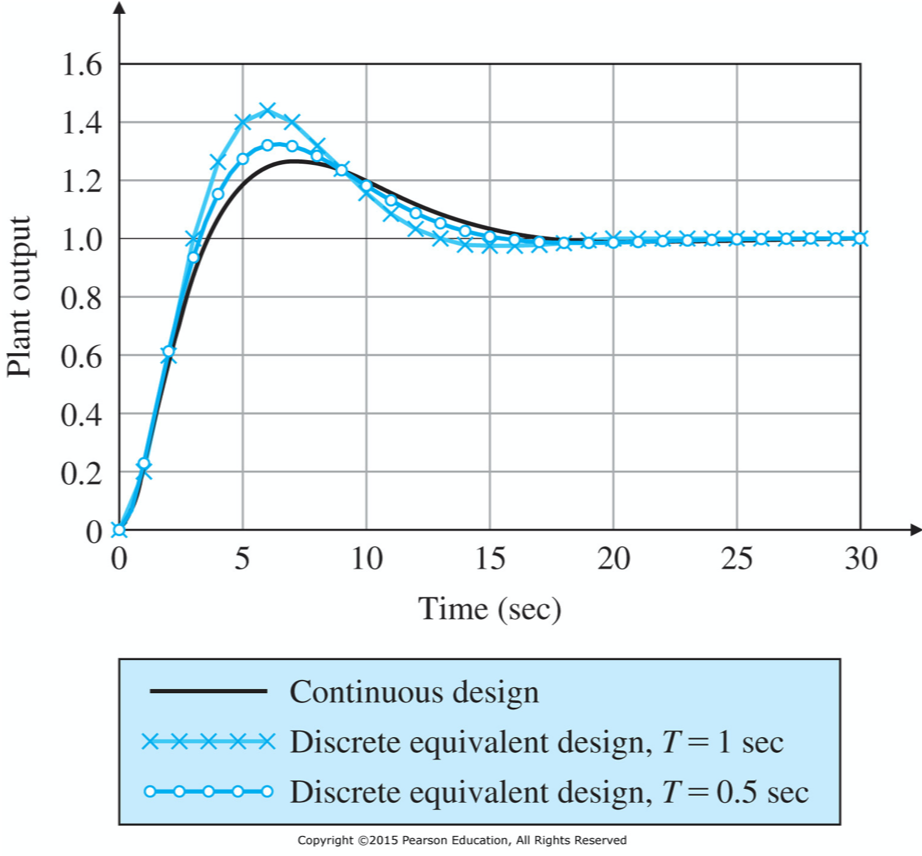
\includegraphics[width=8cm]{./FIG_Franklin/fig8-14.png}
		\end{figure}

\end{itemize}